\documentclass{article}
\usepackage{graphicx}
\usepackage[paper=a4paper, margin=15mm]{geometry}
\usepackage[utf8]{inputenc}
\usepackage{hyperref}
\hypersetup{colorlinks=true, linkcolor=blue, filecolor=magenta, urlcolor=cyan}
 
\urlstyle{same}

\newcommand{\code}[1]{\mbox{\texttt{#1}}}
\newcommand{\refXs}{\code{ref\_X$^*$}}
\newcommand{\sigI}{\code{sig\_I}}

\newlength{\figWidthTab}
\setlength{\figWidthTab}{.9\textwidth}

\title{STUDENT USER MANUAL\\~\\Arduino lock-in amplifier}
\title{ARDUINO LOCK-IN AMPLIFIER\\~\\Student user manual}
\author{Dr. ir. Dennis P.M. van Gils}
\date{\today}

\begin{document}

% --------------------------------------------------------------
%
%   TITLE PAGE
%
% --------------------------------------------------------------

\maketitle
\pagenumbering{gobble}
\centerline{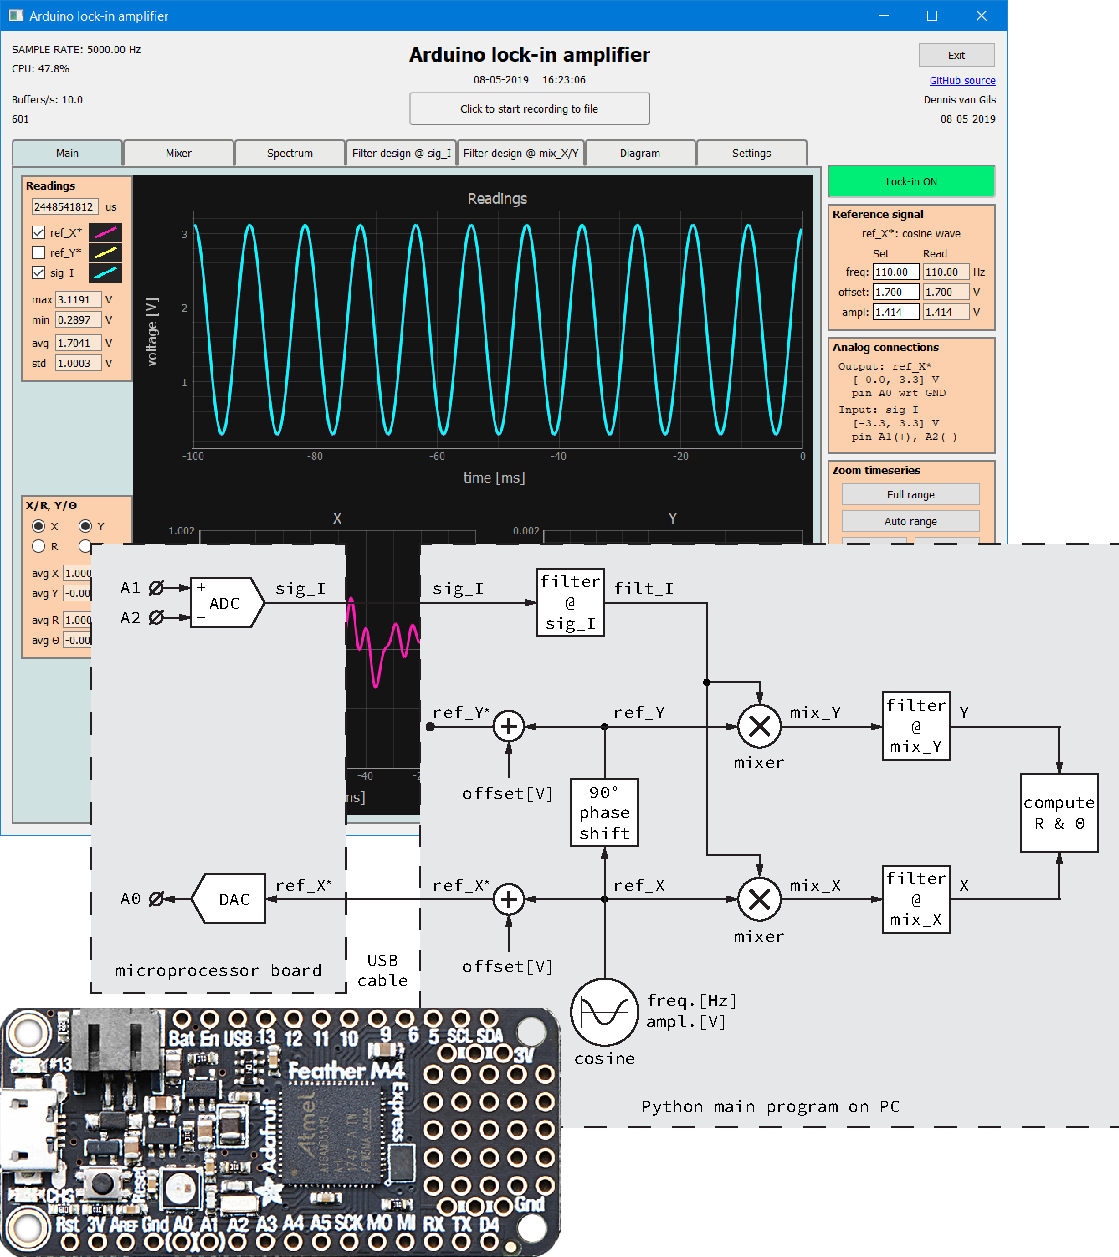
\includegraphics[width=\textwidth]{cover_image.pdf}}

% --------------------------------------------------------------
%
%   TABLE OF CONTENTS
%
% --------------------------------------------------------------

\newpage
\newgeometry{top=1.5in, bottom=1in, right=1.5in, left=1.5in}
\tableofcontents

% --------------------------------------------------------------
%
%   SECTION: Introduction
%
% --------------------------------------------------------------

\newpage
\pagenumbering{arabic}

\section{Introduction}

This document describes a lock-in amplifier running on an Adafruit M4 Feather Express microcontroller board in combination with a PC running Python. It is part of the lab assignments of the course \textit{'Small Signals \& Detection'} of the University of Twente, Enschede, The Netherlands.

The microcontroller (MCU) board generates the reference signal \refXs{} and subsequently acquires the input signal \sigI{}. This data is sent over USB to a PC running the main graphical user interface in Python. The Python program shows the waveform graphs of the signals in real-time, performs the heterodyne mixing and filtering of the signals similar to a lock-in amplifier, and provides logging to disk.

\bigskip\noindent
Current specifications MCU:
\begin{itemize}
\item{Support for Atmel SAMD21 or SAMD51 chipsets}
\item{True analog-out waveform generator (\refXs{} between 0 to 3.3 V)}
\item{Differential analog-in data acquisition (\sigI{} between -3.3 to 3.3 V)}
\item{The DAC (digital-to-analog converter) and ADC (analog-to-digital converter) operate at 12 bits resolution at a sample rate of 5 kHz}
\item{Double-buffered binary-data transmission over USB to a PC running Python}
\end{itemize}

\bigskip\noindent
Current specifications Python:
\begin{itemize}
\item{Separate computing threads for real-time communication with the MCU, signal processing and graphing}
\item{Automatic detection of the MCU board by scanning over all COM ports}
\item{High-quality zero-phase distortion linear FIR filters}
\item{Optional OpenGL hardware-accelerated graphing}
\item{Data logging to file}
\end{itemize}

% --------------------------------------------------------------
%
%   SECTION: Software installation
%
% --------------------------------------------------------------

\newpage
\section{Software installation}

\subsection{Python distribution}
The preferred Python distribution is Anaconda Python 3.7 which can be found at:\\
\href{https://www.anaconda.com/distribution/}{https://www.anaconda.com/distribution/}

\bigskip\noindent
Install Anaconda Python on your laptop. When the installation is finished, start up Anaconda Navigator and install the packages \code{pyserial}, \code{pyqtgraph} and \code{pyopengl} in the environment. Alternatively, the packages can also be installed using the Anaconda Prompt window and entering the following commands:
\begin{verbatim}
conda install pyserial
conda install pyqtgraph
conda install pyopengl
\end{verbatim}

\subsection{GitHub source}\label{sub:GitHub}
Download the source files from the GitHub site of Dennis van Gils at:\\
\href{https://github.com/Dennis-van-Gils/DvG_Arduino_lock-in_amp/}{https://github.com/Dennis-van-Gils/DvG\_Arduino\_lock-in\_amp/}

\bigskip\noindent
Click on the green button labeled \textit{'Clone or download'} and chose \textit{'Download ZIP'}. Extract the \code{zip}-file. This will create the folder:
\begin{verbatim}
<Download folder>\DvG_Arduino_lockin_amp-master
\end{verbatim}

\subsection{M4 Feather Express drivers and firmware}
When using Windows install the Adafruit device drivers at:\\
\href{https://github.com/adafruit/Adafruit_Windows_Drivers/releases/download/2.3.4/adafruit_drivers_2.3.4.0.exe}{https://github.com/adafruit/Adafruit\_Windows\_Drivers/releases/}

\bigskip\noindent
Before the M4 Feather Express can be used as a lock-in amplifier it needs to be flashed with the correct firmware, once. This is already done for you. In case you need to do it again follows here the procedure:

\bigskip\noindent
Connect the M4 Feather Express via USB to your laptop. Quickly double-click on the tiny reset button of the M4 board. The LED on the board should turn green as indication that we have entered Bootloader Mode. Once the bootloader is running, check your computer. You should see a USB Disk drive called \code{'FEATHERBOOT'}. This folder contains the file \code{CURRENT.UF2} which is the current contents of the microcontroller flash. You can upload new firmware to the M4 board by copying over this file. The lock-in amplifier firmware can be found in the downloaded GitHub source files from \S \ref{sub:GitHub} in folder:
\begin{verbatim}
\source_MCU_boards\pre-compiled_M4_feather
\end{verbatim}
The M4 board should automatically reboot when the file is copied over and will now be running the lock-in amplifier firmware.

\subsection{Running the main program}
Connect the M4 Feather Express via USB to your laptop. Start the Anaconda Prompt window and change the folder to: \begin{verbatim}
<Download folder>\DvG_Arduino_lockin_amp-master
\end{verbatim}

\bigskip\noindent
Now run the following command in the prompt:
\begin{verbatim}
ipython DvG_Arduino_lockin_amp.py
\end{verbatim}

\noindent
This will start a user interface in which you can configure and control your measurements.

% --------------------------------------------------------------
%
%   SECTION: Hardware information
%
% --------------------------------------------------------------

\newpage
\section{Hardware information}
The Adafruit Feather M4 Express microcontroller board features a 120 MHz Cortex M4 with floating point support and 512 KB of Flash and 192 KB of RAM memory.

In the current lock-in amplifier firmware the DAC (digital-to-analog converter) and ADC (analog-to-digital converter) are set to operate at 12 bits resolution at a sample rate of 5 kHz. The frequency of the output reference signal \refXs{} is limited to 5 kHz / 4 = 1250 Hz.

\begin{figure}[h]\label{fig:pinout}
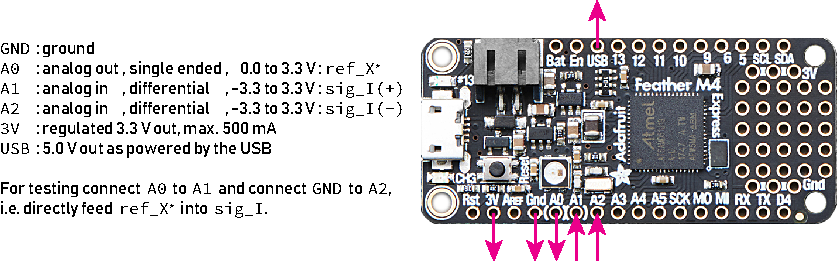
\includegraphics[width=\textwidth]{pinout_Adafruit_Feather_M4_Express.pdf}
\caption{Pinout of the Adafruit Feather M4 Express microprocessor board.}
\end{figure}

% --------------------------------------------------------------
%
%   SECTION: Signal processing
%
% --------------------------------------------------------------

\section{Signal processing}

\begin{figure}[h]\label{fig:diagram}
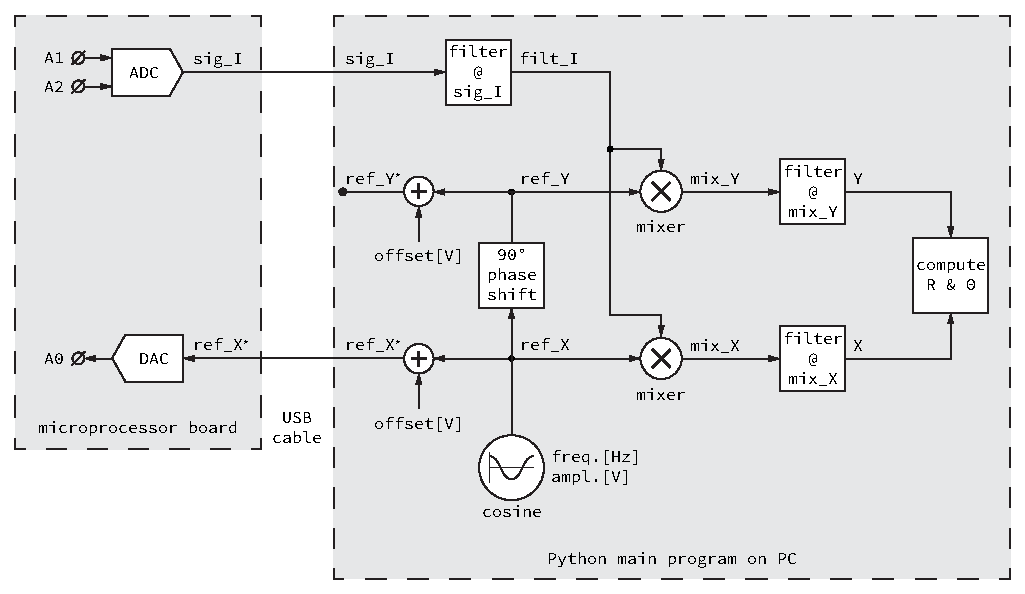
\includegraphics[width=\textwidth]{diagram_signal_processing.pdf}
\caption{Diagram of the signal processing steps making up a fully functioning lock-in amplifier.}
\end{figure}

% --------------------------------------------------------------
%
%   SECTION: Python GUI
%
% --------------------------------------------------------------

\newpage
\section{Python GUI}
This section describes the graphical user interface (GUI) of the lock-in amplifier running in Python.

\begin{figure}[h]\label{fig:tab_1}
\centering
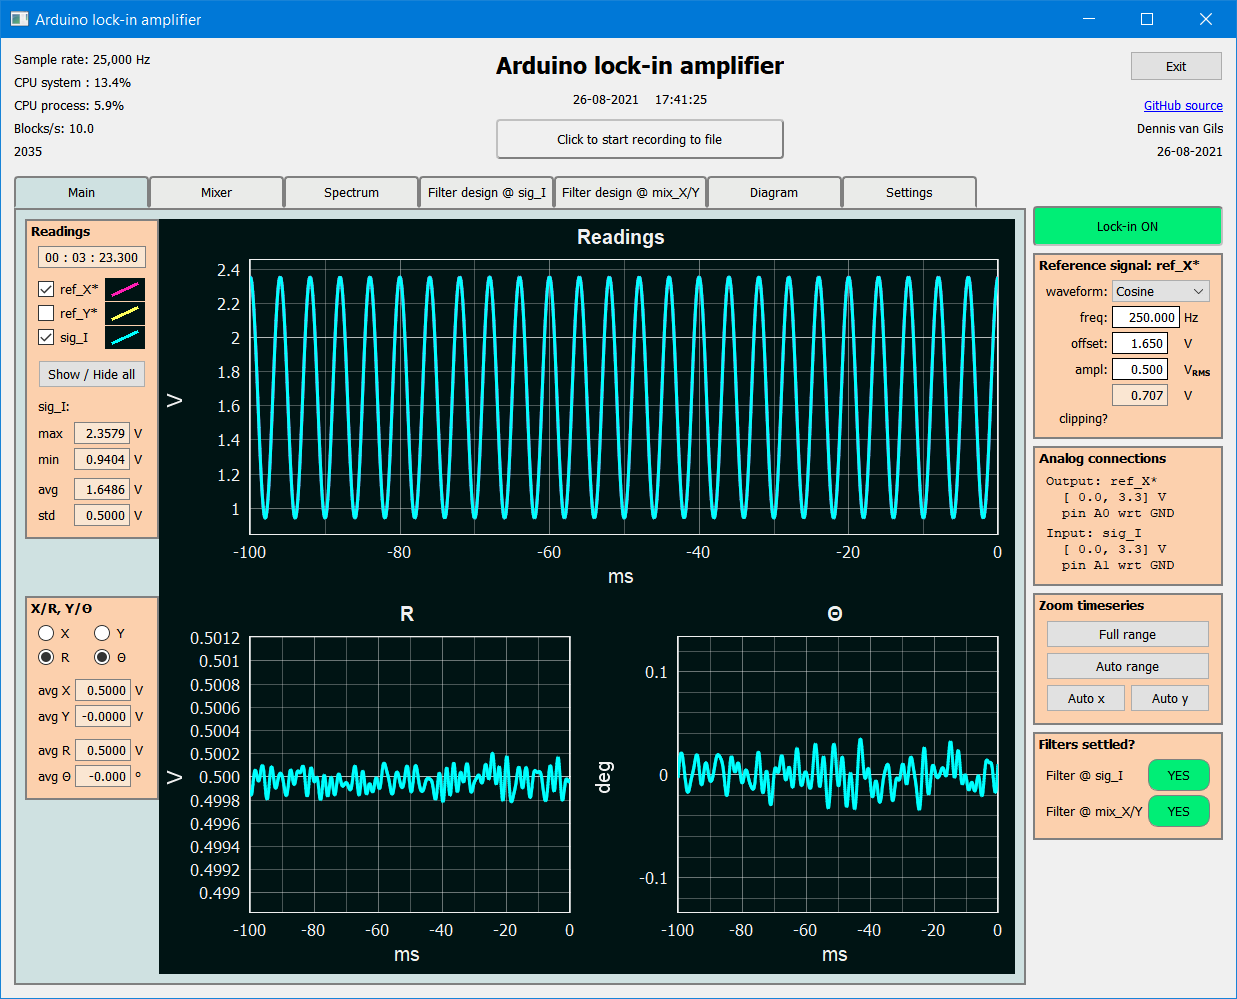
\includegraphics[width=\figWidthTab]{tab_1.PNG}
\caption{The \textit{Main} tab page of the lock-in amplifier GUI.}
\end{figure}

\begin{figure}[h]\label{fig:tab_2}
\centering
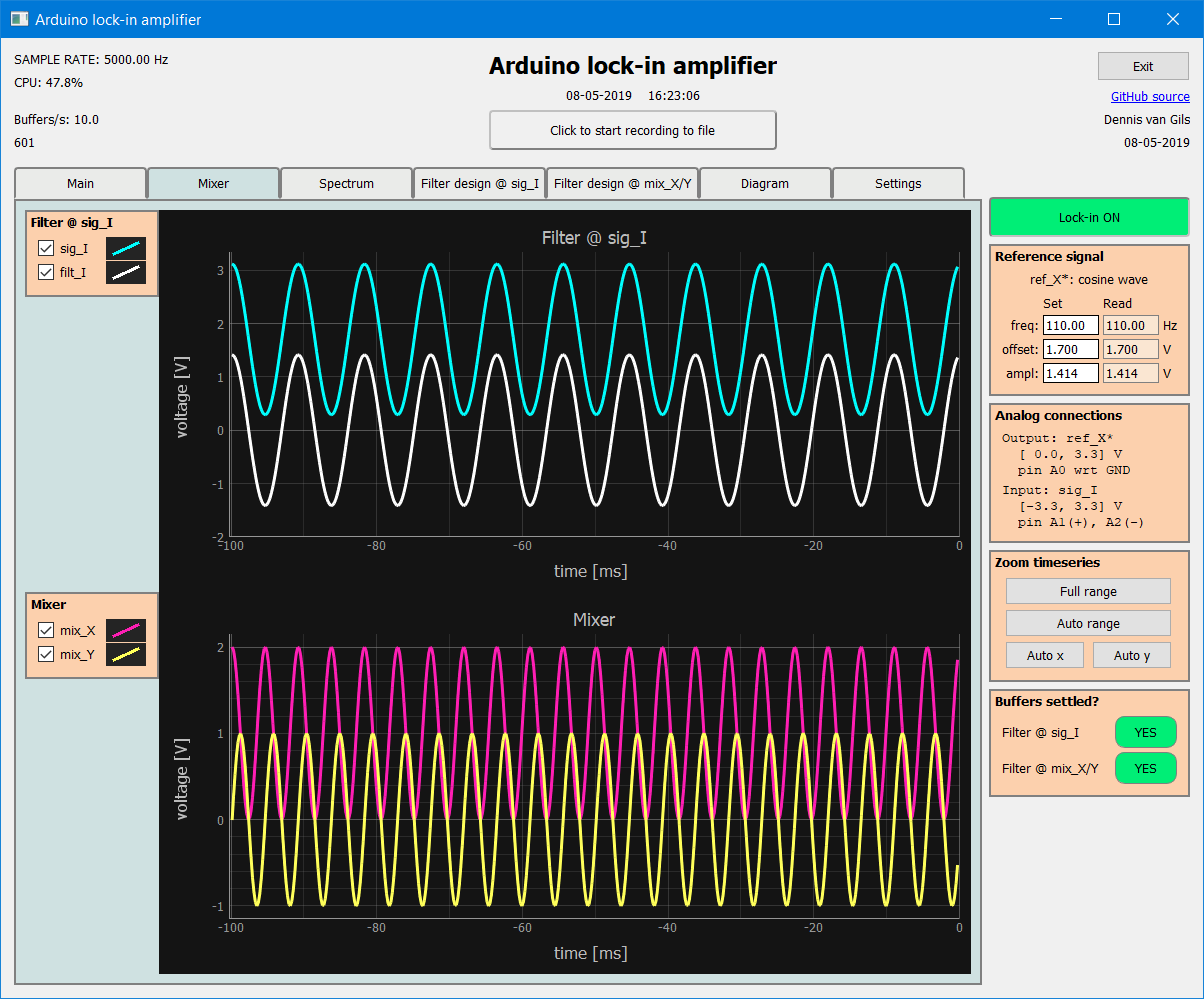
\includegraphics[width=\figWidthTab]{tab_2.PNG}
\caption{The \textit{Mixer} tab page of the lock-in amplifier GUI.}
\end{figure}

\begin{figure}[h]\label{fig:tab_3}
\centering
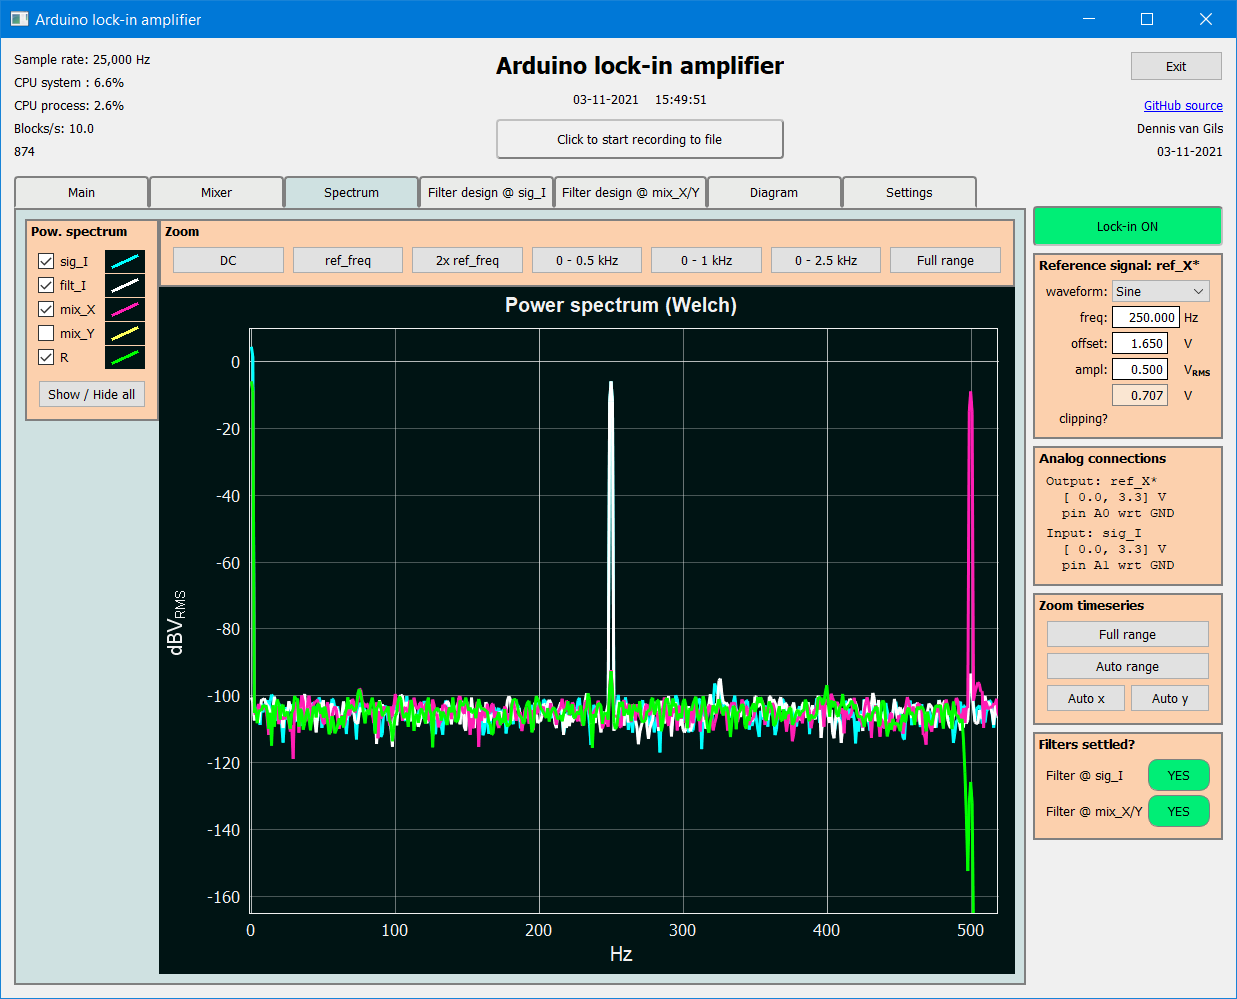
\includegraphics[width=\figWidthTab]{tab_3.PNG}
\caption{The \textit{Spectrum} tab page of the lock-in amplifier GUI.}
\end{figure}

\begin{figure}[h]\label{fig:tab_4}
\centering
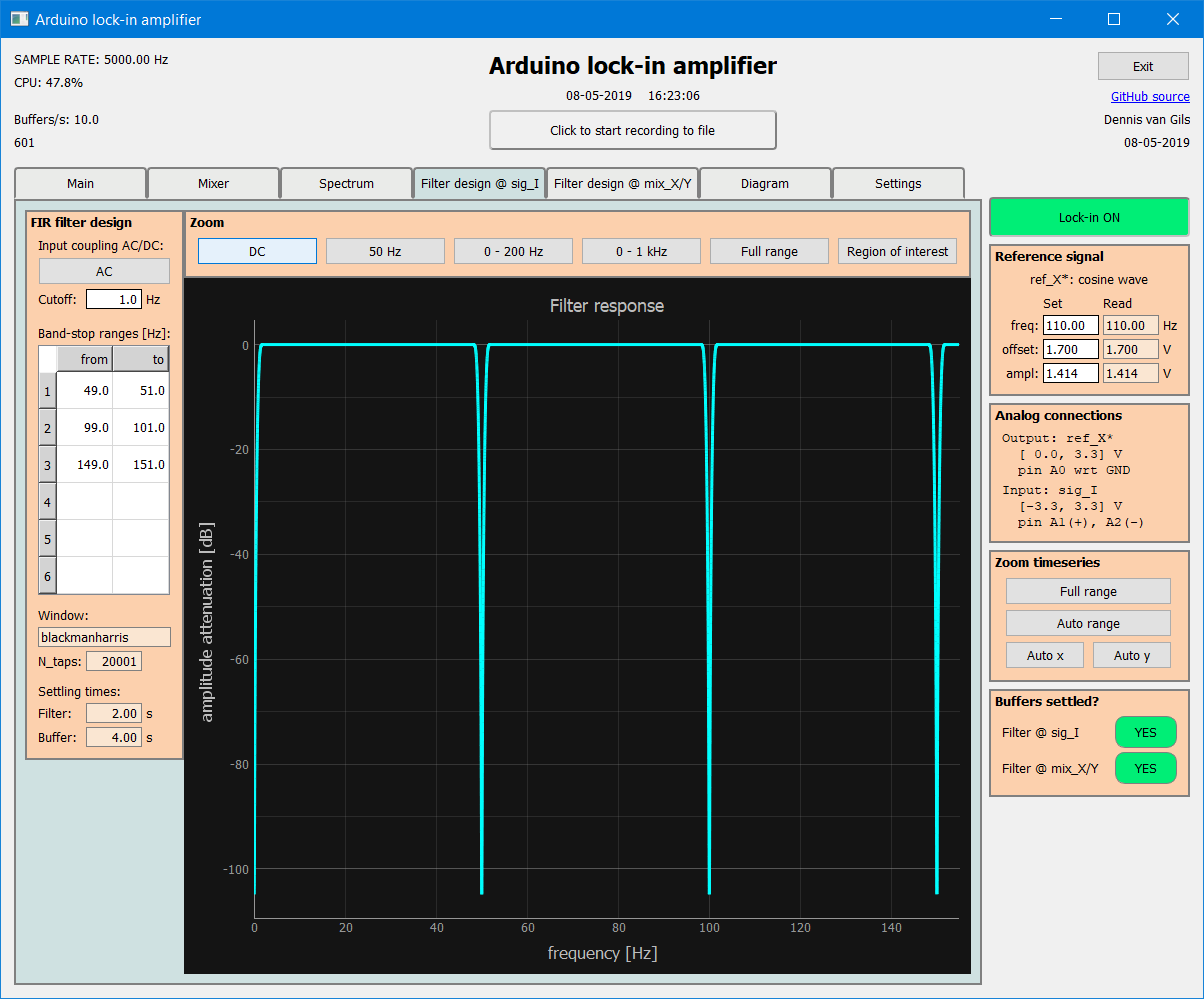
\includegraphics[width=\figWidthTab]{tab_4.PNG}
\caption{The \textit{Filter design @ sig\_I} tab page of the lock-in amplifier GUI.}
\end{figure}

\begin{figure}[h]\label{fig:tab_5}
\centering
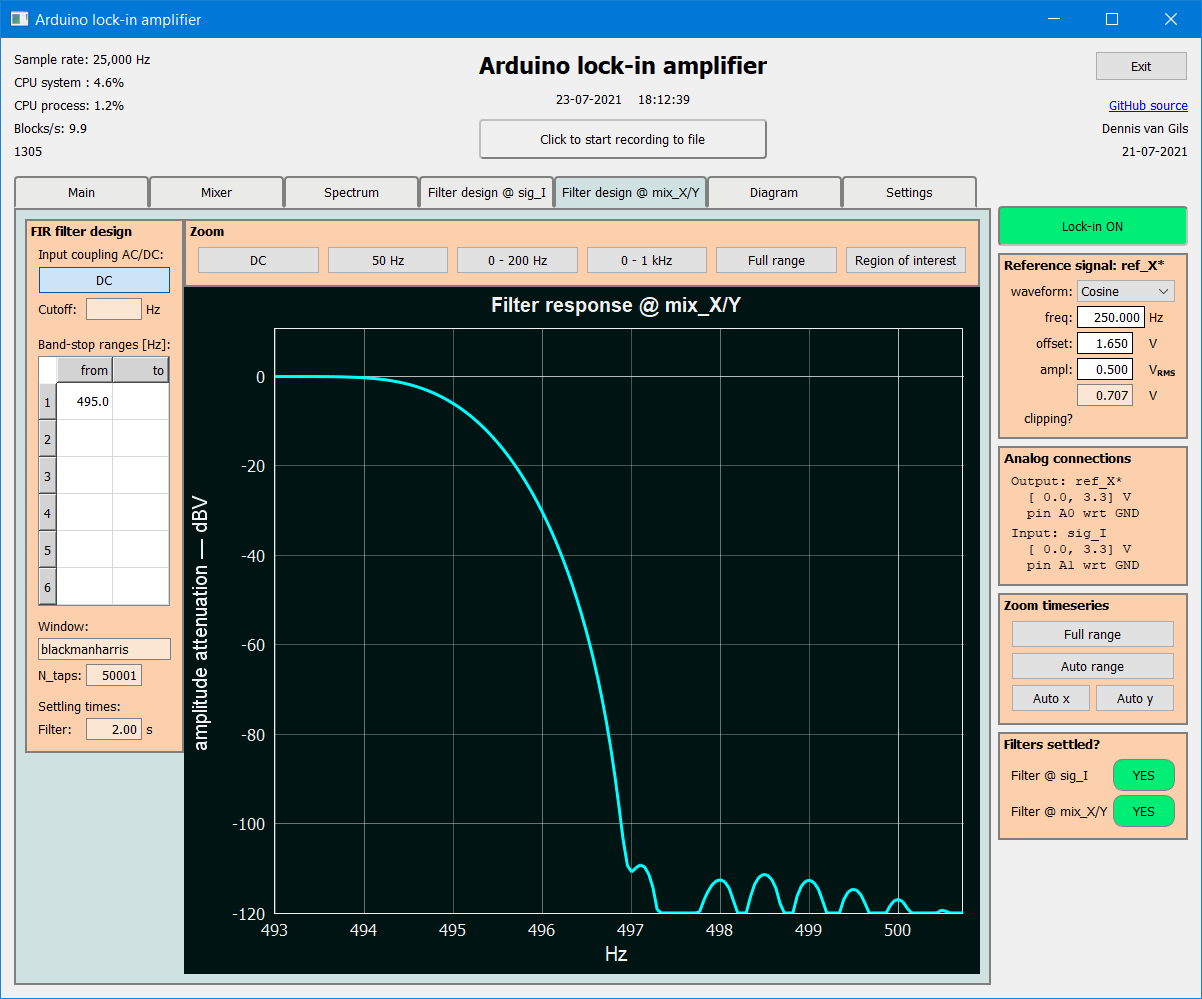
\includegraphics[width=\figWidthTab]{tab_5.PNG}
\caption{The \textit{Filter design @ mix\_X/Y} tab page of the lock-in amplifier GUI.}
\end{figure}

\end{document}
